\documentclass[compress]{beamer}
\usecolortheme{default}

\usepackage{lmodern, epstopdf, multirow, array, setspace, bbm, tcolorbox, pbox, bm, mathtools, tikz}
\usepackage[T1]{fontenc}

\setbeamertemplate{frametitle}[default][center]
\setbeamertemplate{footline}{\hfill \insertframenumber/\inserttotalframenumber\hspace*{5pt}\vspace{5pt}}
\setbeamertemplate{navigation symbols}{}

\newlength{\wideitemsep}
\setlength{\wideitemsep}{\itemsep}
\addtolength{\wideitemsep}{4pt}
\let\olditem\item
\renewcommand{\item}{\setlength{\itemsep}{\wideitemsep}\olditem}
\setlength{\leftmargini}{12pt}
\setlength{\leftmarginii}{14pt}
\setbeamertemplate{itemize/enumerate subbody begin}{\vspace{6pt}}
\setbeamertemplate{itemize item}[circle]
\setbeamertemplate{enumerate item}[circle]
\setbeamertemplate{enumerate subitem}[default]

\setbeamercolor{alerted text}{fg=blue}
\setbeamersize{text margin left=1.5em,text margin right=1.5em}

\tcbset{
    colback=white,
    colframe=black,
    coltext=black,
    coltitle=blue,
    colbacktitle=white,
    boxrule=1pt,
    titlerule=0pt,
    toptitle=4pt,
    top=2pt
}

\newenvironment{changemargin}[2]{% 
  \begin{list}{}{% 
    \setlength{\topsep}{0pt}% 
    \setlength{\leftmargin}{#1}% 
    \setlength{\rightmargin}{#2}% 
    \setlength{\listparindent}{\parindent}% 
    \setlength{\itemindent}{\parindent}% 
    \setlength{\parsep}{\parskip}% 
  }% 
  \item[]}{\end{list}}
  
\newenvironment{defn}{%
  \begin{tcolorbox}[title={Definition}]%
  }{\end{tcolorbox}}
  
\newenvironment{prop}[1]{%
  \begin{tcolorbox}[title={Proposition #1}]%
  }{\end{tcolorbox}}
  
\newcommand{\cit}[1]{{\footnotesize \textcolor[rgb]{0.5,0,0}{#1}}}

% Font size for code listings (verbatim blocks); reset with \normalsize
\newcommand{\codesize}{\fontsize{7}{8.5}\selectfont}

\newcommand{\slidesetup}[1]{%
  \title{#1}%
  \subtitle{\texorpdfstring{\vspace{0.3\baselineskip}}{} {\small This version: \today}}%
  \author[Mikkel Plagborg-Moller]{ECMA 31150, Spring 2026 \texorpdfstring{\\[0.5ex]}{} University of Chicago \texorpdfstring{\\[0.5ex]}{} Department of Economics \texorpdfstring{\\[4ex]}{} Mikkel Plagborg-Moller}%
  \date{}%
}

% \circleoverlay[options]{text}
% Draws a red circle with a text box nearby on a tikz overlay.
% Options (with defaults):
%   cx=0cm, cy=0cm      - circle center (shift from page center)
%   r=1cm               - circle radius
%   tx=0cm, ty=0cm      - text box offset from circle center
%   text anchor=east    - anchor of text node (east = text left, west = text right)
%   font=\normalsize    - font size for text
\pgfkeys{
  /circleoverlay/.cd,
  cx/.store in=\cocx, cx=0cm,
  cy/.store in=\cocy, cy=0cm,
  r/.store in=\cor, r=1cm,
  tx/.store in=\cotx, tx=0cm,
  ty/.store in=\coty, ty=0cm,
  text anchor/.store in=\cotextanchor, text anchor=east,
  font/.store in=\cofont, font=\normalsize,
}
\newcommand{\circleoverlay}[2][]{%
  \pgfkeys{/circleoverlay/.cd, cx=0cm, cy=0cm, r=1cm, tx=0cm, ty=0cm, text anchor=east, font=\normalsize, #1}%
  \pgfmathsetlengthmacro{\circlediameter}{2*\cor}%
  \node[draw=red, line width=2pt, circle, minimum size=\circlediameter, inner sep=0pt]
    (tmpcirc) at ([xshift=\cocx,yshift=\cocy]current page.center) {};%
  \node[anchor=\cotextanchor, fill=white, draw=red, text=red, inner sep=4pt, align=left, font=\cofont]
    at ([xshift=\cotx,yshift=\coty]tmpcirc.center) {#2};%
}

\DeclareMathOperator*{\argmax}{argmax}
\DeclareMathOperator*{\argmin}{argmin}
\DeclareMathOperator{\diag}{diag}
\DeclareMathOperator{\var}{Var}
\DeclareMathOperator{\cov}{Cov}
\DeclareMathOperator{\corr}{Corr}
\DeclareMathOperator{\lrv}{LRV}


\slidesetup{Non-stationary models I}

\begin{document}
\frame{
\maketitle
}

\frame{
\frametitle{Plan for this slide deck}
\begin{enumerate}
\item Models for trending data
\item What happens if we try to estimate a non-stationary AR model by OLS?
\item How can we test the stationarity assumption?
\item Should we even try to categorize series as stationary or non-stationary?
\end{enumerate}
}

\frame{
\frametitle{Trending data}
\begin{itemize}
\item As we've seen many times, lots of economic time series exhibit clear trends over time.
\item This makes them \textbf{non-stationary}.
\item So far we've primarily been dealing with this by transforming the data to stationarity, e.g., by differencing.
\item But what if we care about the trends \emph{per se}? And even if we don't, are we losing statistical power by transforming the data?
\end{itemize}
}

\frame{
\begin{figure}
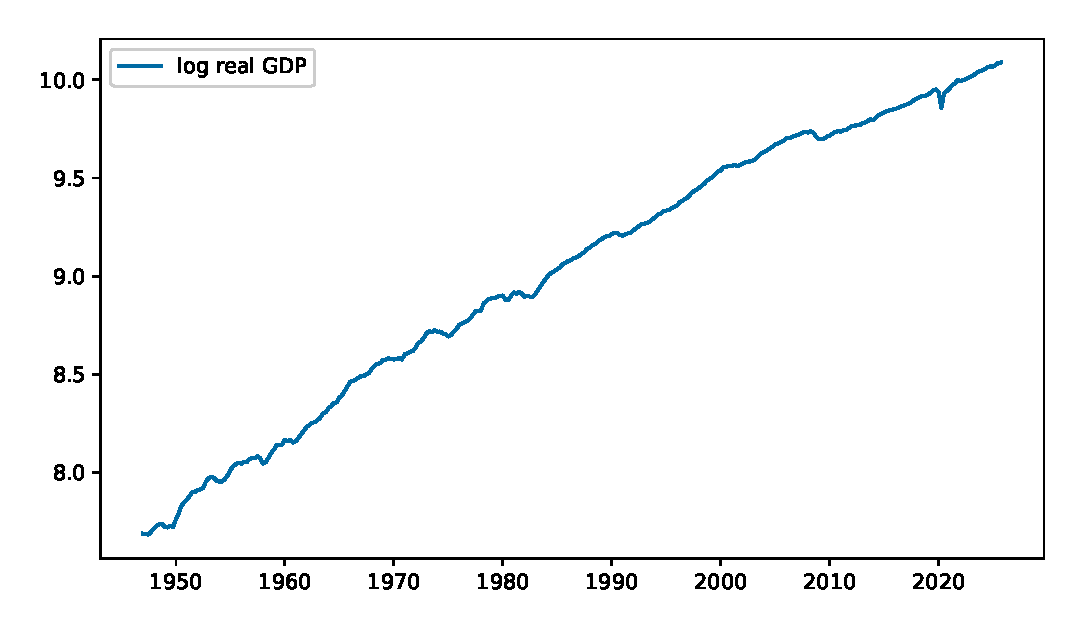
\includegraphics[width=\linewidth]{fig/lgdp.eps}
\end{figure}
}

\frame{
\frametitle{Trend stationarity}
\begin{itemize}
\item One approach to trends is to model the data as arising from stationary fluctuations around a \textbf{deterministic time trend}:
\[y_t = \underbrace{\beta_0 + \beta_1 t}_\text{deterministic} + v_t,\]
where $\lbrace v_t \rbrace$ is stationary and weakly dependent.
\item We say that $\lbrace y_t \rbrace$ is \textbf{trend stationary}.
\item The trend need not be linear:
\[y_t = \beta_0 + \beta_1 t + \beta_2 t^2 + \dots + \beta_p t^p + v_t.\]
\end{itemize}
}

\begin{frame}[fragile]
\small
\begin{verbatim}
# Trend regression
y = l_gdp.values
T = y.shape[0]
trend = np.arange(T)

# Linear
X_lin = sm.add_constant(trend)
res_lin = sm.OLS(y, X_lin).fit()

# Quadratic
X_quad = sm.add_constant(np.column_stack([trend, trend**2]))
res_quad = sm.OLS(y, X_quad).fit()
\end{verbatim}
\end{frame}

\frame{
\begin{figure}
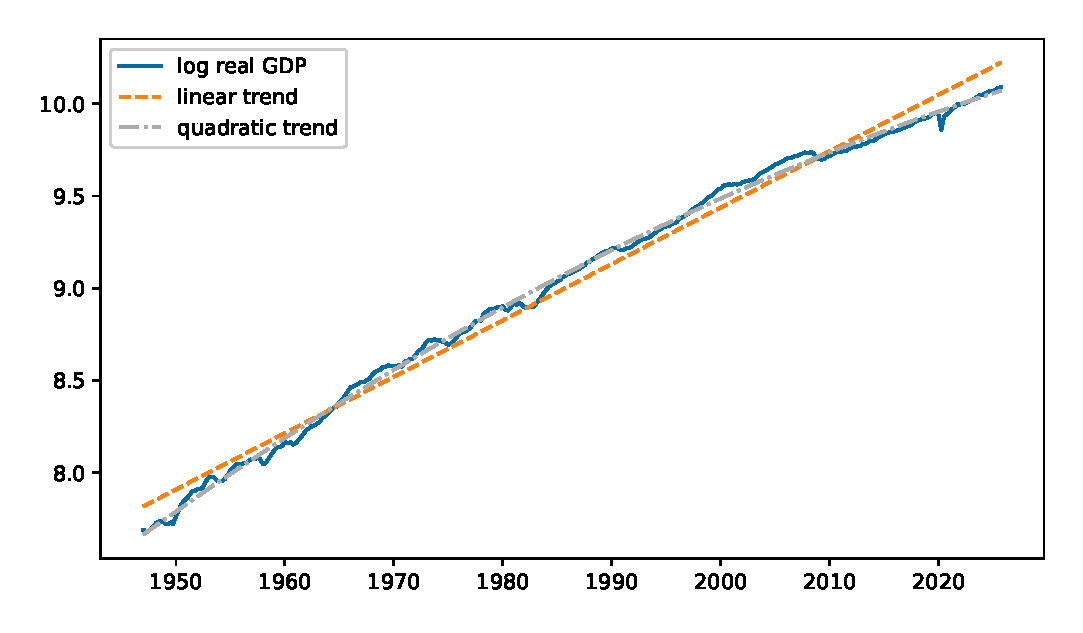
\includegraphics[width=\linewidth]{fig/lgdp_trend.eps}
\end{figure}
}

\frame{
\frametitle{Trend stationarity: forecasting}
\begin{itemize}
\item Optimal $h$-step forecast of a trend stationary series:
\begin{align*}
&E[y_{T+h} \mid y_T,y_{T-1},\dots] \\
&= \underbrace{\beta_0 + \beta_1 (T+h) + \dots + \beta_p (T+h)^p}_\text{no uncertainty} + E[v_{T+h} \mid y_T,y_{T-1},\dots],
\end{align*}
with MSFE
\[\var(y_{T+h} \mid y_T,y_{T-1},\dots) = \var(v_{T+h} \mid y_T,y_{T-1},\dots).\]
\item The trend itself does not contribute at all to the MSFE (apart from parameter estimation error), since we can extrapolate out of sample based on the deterministic functional form.
\end{itemize}
}

\frame{
\frametitle{Trend stationarity: forecasting (cont.)}
\[\var(y_{T+h} \mid y_T,y_{T-1},\dots) = \var(v_{T+h} \mid y_T,y_{T-1},\dots)\]
\begin{itemize}
\item If $\lbrace v_t \rbrace$ is stationary and weakly dependent, then as the forecast horizon $h \to \infty$, we have $\var(v_{T+h} \mid y_T,y_{T-1},\dots) \to \var(v_t)$.
\item Hence, the MSFE for a trend stationary series $\lbrace y_t \rbrace$ stabilizes at long horizons $h \to \infty$, rather than growing without bound.
\item This seems implausible -- in practice, we're very uncertain about the level of real GDP 10 years from now, say.
\item Trend stationary models are also prone to \textbf{overfitting}: with a high polynomial order $p$, we can fit trends well \emph{in sample}, but may do very poorly \emph{out of sample}.
\end{itemize}
}

\frame{
\begin{figure}
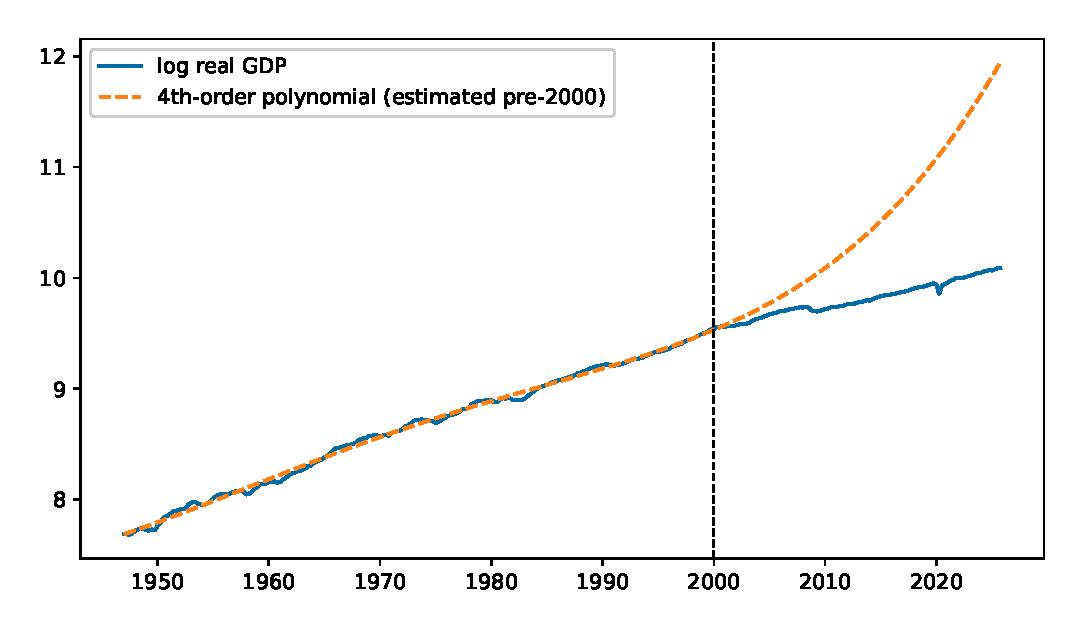
\includegraphics[width=\linewidth]{fig/lgdp_poly.eps}
\end{figure}
}

\frame{
\frametitle{Stochastic trends}
\begin{itemize}
\item Deterministic trends are unrealistic. We would like a model with a \textbf{stochastic trend}.
\item A building block model is the \textbf{random walk}:
\[y_t = y_{t-1} + u_t,\quad u_t \overset{iid}{\sim} (0,\sigma^2).\]
This is an AR(1) model with $\rho=1$.
\item Note:
\[y_t = u_t + u_{t-1} + \dots + u_1 + y_0 = y_0 + \sum_{s=1}^t u_s.\]
\item If we treat the initial condition $y_0$ as a random variable independent of $\lbrace u_t \rbrace$, then
\[\var(y_t) = \var(y_0) + t\sigma^2 \to \infty \quad \text{as } t\to\infty.\]
\end{itemize}
}

\frame{
\begin{figure}
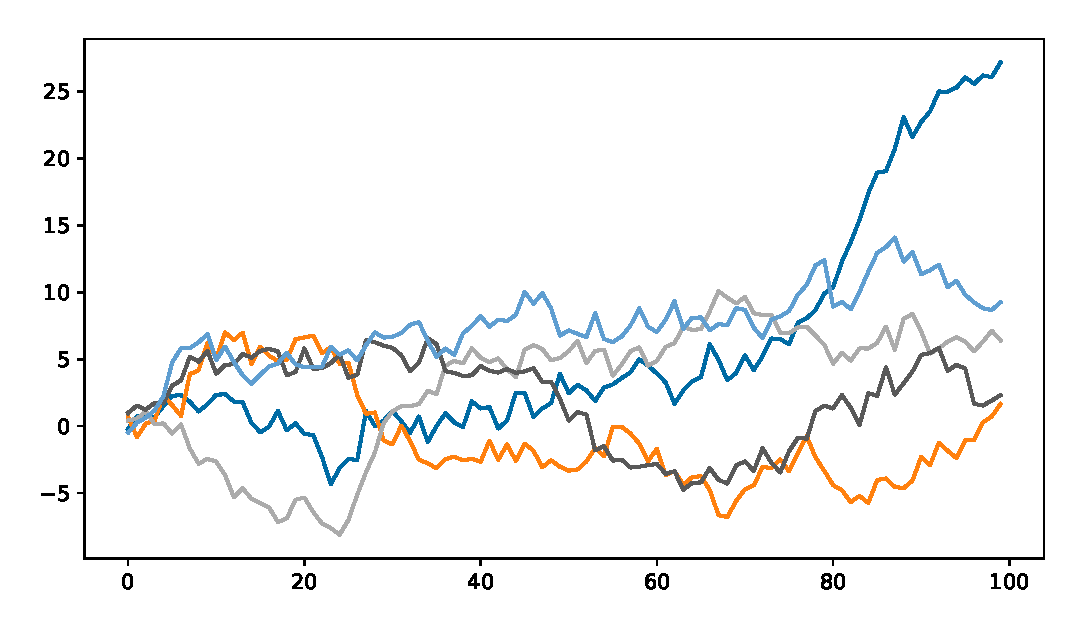
\includegraphics[width=\linewidth]{fig/rw_sim.eps} \\
\bigskip
5 sample paths of random walks with $u_t \overset{iid}{\sim} N(0,1)$ and $y_0=0$ \\
\smallskip
Notice: some paths exhibit apparent trends, but not deterministic
\end{figure}
}

\frame{
\frametitle{Random walk: forecasting}
\[y_t = y_{t-1} + u_t,\quad u_t \overset{iid}{\sim} (0,\sigma^2)\]
\vspace{-0.5\baselineskip}
\begin{itemize}
\item For a random walk, the optimal forecast is ``no change'', both in the short and long run:
\[E[y_{T+h} \mid y_T,y_{T-1},\dots] = E\left[y_T + \sum_{\ell=1}^h u_{T+\ell} \;\Bigg|\; y_T,y_{T-1},\dots\right] = \boxed{y_T}.\]
\item MSFE is linearly increasing in the forecast horizon $h$:
\[\var(y_{T+h} \mid y_T,y_{T-1},\dots) = \var\left(\sum_{\ell=1}^h u_{T+\ell}\right) = \boxed{h\sigma^2}.\]
More realistic than trend stationary models.
\end{itemize}
}

\frame{
\frametitle{Random walk with drift}
\begin{itemize}
\item The pure random walk is equally likely to exhibit increasing or decreasing stochastic trends.
\item We can introduce a positive \textbf{drift} in $\lbrace y_t \rbrace$ by introducing an intercept:
\[y_t = c + y_{t-1} + u_t,\quad u_t \overset{iid}{\sim} (0,\sigma^2)\]
\[\Longrightarrow\quad y_t = y_0 + \underbrace{\vphantom{\sum_{s=1}^t}ct}_\text{deterministic trend} + \underbrace{\sum_{s=1}^t u_s}_\text{stochastic trend}.\]
\item Long-run forecasts remain very uncertain (\alert{exercise:} verify):
\[\var(y_{T+h} \mid y_T,y_{T-1},\dots) = \boxed{h\sigma^2}.\]
\end{itemize}
}

\frame{
\begin{figure}
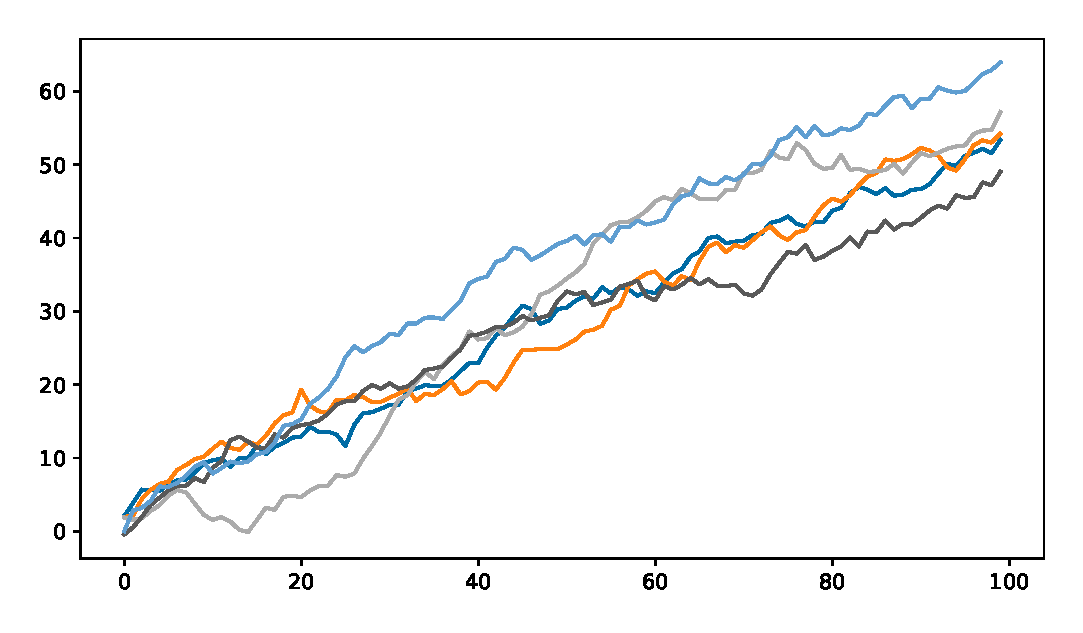
\includegraphics[width=\linewidth]{fig/rw_drift_sim.eps} \\
\vspace{-\baselineskip}
\[c=0.5,\quad u_t \overset{iid}{\sim} N(0,1),\quad y_0=0\]
\end{figure}
}

\frame{
\frametitle{ARIMA}
\begin{itemize}
\item The random walk with drift may be a good description of the long run. But we want a richer model of short-to-medium-run dynamics.
\item Let's assume that $\lbrace y_t \rbrace$ is cov.\ stationary after transforming to first differences $\Delta y_t \equiv y_t-y_{t-1}$.
\item Then we say that $\lbrace y_t \rbrace$ is \textbf{integrated of order 1} or \textbf{I(1)}.
\begin{itemize}
\item If instead $\Delta y_t$ is non-stationary but $\Delta^2y_t \equiv \Delta(\Delta y_t)$ is cov.\ stationary, then we say that $\lbrace y_t \rbrace$ is I(2), and so on.
\end{itemize}
\item Then we can apply our flexible ARMA modeling techniques to the first differences $\Delta y_t$:
\[\tilde{a}(L)(\Delta y_t - \mu) = \theta(L)u_t,\quad u_t \sim \mathit{WN}(\sigma^2).\]
\item \textbf{ARIMA}: AutoRegressive Integrated Moving Average.
\end{itemize}
}

\frame{
\frametitle{ARIMA (cont.)}
\[\tilde{a}(L)(\Delta y_t - \mu) = \theta(L)u_t,\quad u_t \sim \mathit{WN}(\sigma^2),\]
\[\tilde{a}(L) \equiv 1-\sum_{\ell=1}^{p-1} \tilde{a}_\ell L^\ell,\quad \theta(L)\equiv 1 + \sum_{\ell=1}^q \theta_\ell L^\ell.\]
\begin{itemize}
\item Assume $\tilde{a}(L)$ has all roots outside the unit circle, so $\lbrace \Delta y_t \rbrace$ is cov.\ stationary.
\item Random walk with drift is a special case: $\tilde{a}(L)=1$, $\theta(L)=1$, $\mu=c$.
\item The above equation does not fully pin down $y_1,y_2,\dots$; we also need to specify an initial condition $y_0$. Then
\[y_t = y_0 + \sum_{s=1}^t \Delta y_s = y_0 + \underbrace{\mu t}_\text{deterministic trend} + \sum_{s=1}^t \underbrace{(\Delta y_s -\mu)}_\text{stationary}.\]
\end{itemize}
}

\frame{
\frametitle{Autoregression with unit root}
\begin{itemize}
\item Consider an ARIMA model with $\theta(L)=1$. Then, since $\Delta \equiv 1-L$,
\[\tilde{a}(L)(\Delta y_t - \mu) = u_t,\quad u_t \sim \mathit{WN}(\sigma^2)\]
\[\Longrightarrow \quad a(L)y_t = c + u_t,\quad \text{where } a(L)\equiv (1-L)\tilde{a}(L),\; c \equiv \tilde{a}(1)\mu.\]
\item This is an AR($p$) model (since we assumed $\tilde{a}(L)$ is of order $p-1$).
\item One of the roots of the AR polynomial $a(L)$ is equal to 1:
\[a(1) = (1-1)\tilde{a}(1) = 0.\]
We call this an autoregression with a \textbf{unit root}.
\item The random walk with drift is an AR(1) with a unit root:
\[\underbrace{(1-L)}_{a(L)}y_t = c + u_t \quad \Longrightarrow \quad a(1)=0.\]
\end{itemize}
}

\frame{
\frametitle{Autoregression with unit root (cont.)}
\[a(L)y_t = c + u_t,\quad a(L) \equiv 1-\sum_{\ell=1}^p a_\ell L^\ell\]
\begin{itemize}
\item The AR($p$) process has a unit root if and only if the sum of the autoregressive coefficients equals 1:
\[a(1)=0 \quad \Longleftrightarrow \quad 1- \sum_{\ell=1}^p a_\ell \times 1^\ell = 0 \quad \Longleftrightarrow\quad \boxed{\sum_{\ell=1}^p a_\ell = 1}.\]
\end{itemize}
}

\frame{
\begin{figure}
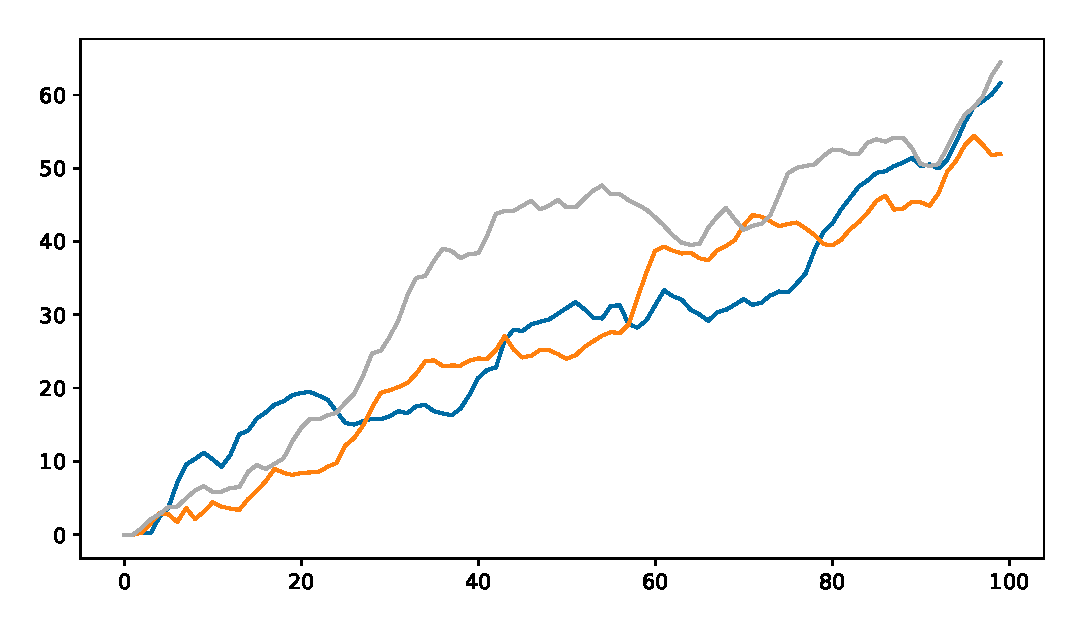
\includegraphics[width=\linewidth]{fig/unitroot_ar2_sim.eps}
\[y_t = 0.3 + 1.5y_{t-1} - 0.5y_{t-2} + u_t,\quad u_t \overset{iid}{\sim} N(0,1)\]
\end{figure}
}

\frame{
\frametitle{Estimation with stochastic trends}
\begin{itemize}
\item If we are certain that a time series has a stochastic trend, then we can fit an AR/ARMA model in first differences.
\item But sometimes we don't know \emph{a priori} whether to model a series as trending or stationary (but persistent).
\item We may want to \emph{test} whether the series has a stochastic trend.
\end{itemize}
}

\frame{
\frametitle{OLS estimation with a unit root}
\begin{itemize}
\item Suppose we estimate an AR(1) model by OLS:
\[y_t = \hat{c} + \hat{\rho} y_{t-1} + \hat{u}_t.\]
\item If the true AR(1) process has $|\rho|<1$, then we know that $\hat{\rho}$ and associated t-statistic are normally distributed in large samples.
\item But if the true process has a unit root, then this is no longer the case!
\item Next slide: simulated sampling distributions of $\hat{\rho}$ when true $\rho$ equals 0.7 and 1, respectively.
\end{itemize}
}

\frame{
\begin{figure}
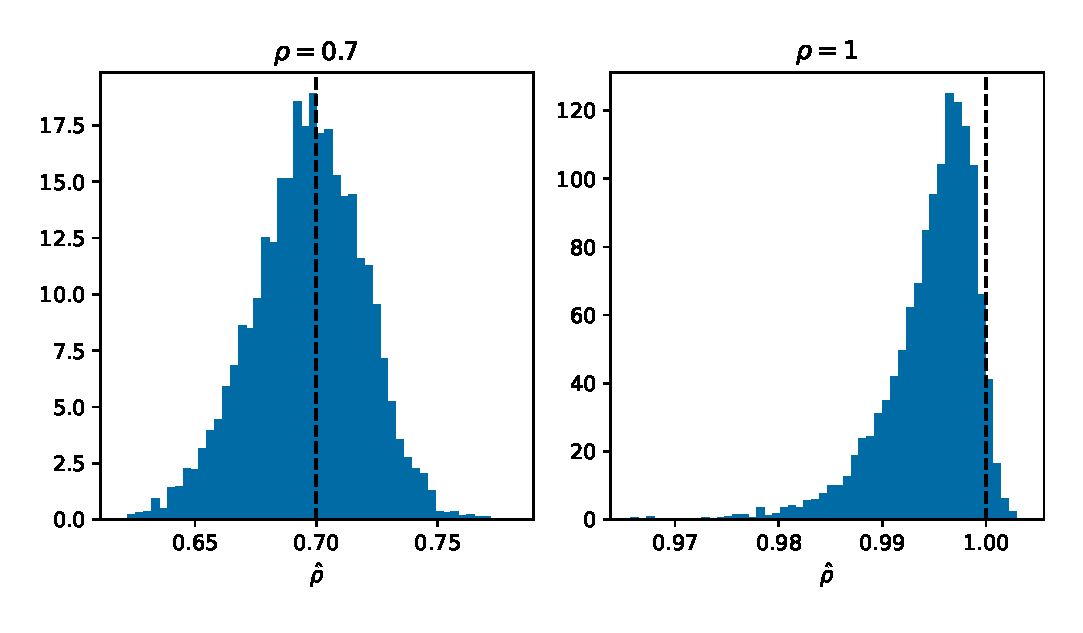
\includegraphics[width=\linewidth]{fig/unitroot_mc.eps} \\
\vspace{-\baselineskip}
\[y_t = \rho y_{t-1} + u_t,\quad u_t \overset{iid}{\sim} N(0,1),\quad T=1000,\quad 5000 \text{ simulations}\]
\smallskip
Notice the different axis scales
\end{figure}
}

\frame{
\frametitle{OLS estimation with a unit root (cont.)}
\begin{itemize}
\item In the unit root case $\rho=1$, the large-$T$ sampling distribution of $\hat{\rho}$ is left-skewed and definitely not normal.
\item The distribution is highly concentrated, though: $\var(\hat{\rho})$ is very small.
\item Intuitively, we know that $\hat{\rho}$ is biased downward in finite samples. The bias is increasing in the persistence $\rho$. As $\rho \to 1$, the bias is no longer negligible relative to the (small) standard deviation of $\hat{\rho}$.
\item $\hat{\rho}$ remains \emph{consistent} for $\rho=1$ as $T \to \infty$. In fact, it's \textbf{super-consistent}: its standard deviation decreases at rate $\boxed{1/T}$, not $1/\sqrt{T}$ as we're used to.
\item Summary: when $\rho=1$, $\hat{\rho}$ is highly precise, but its distribution is asymmetric. Invalidates conventional SE and confidence interval.
\end{itemize}
}

\frame{
\frametitle{Unit root test}
\[y_t = c + \rho y_{t-1} + u_t\]
\begin{itemize}
\item Suppose we want to test the null hypothesis that $\lbrace y_t \rbrace$ is a random walk without drift ($\rho=1$, $c=0$) against the stationary alternative ($|\rho|<1$, $c$ arbitrary).
\item It's natural to compute the OLS estimator $\hat{\rho}$ and the t-statistic
\[\hat{t} \equiv \frac{\hat{\rho}-1}{\mathit{SE}(\hat{\rho})},\]
where the denominator is the usual SE formula for OLS computed under \emph{homoskedasticity} (will explain soon).
\item If we find $\hat{t}$ to be very negative, we ought to reject the unit root hypothesis; otherwise we can't reject. How negative?
\end{itemize}
}

\frame{
\frametitle{Unit root test (cont.)}
\[\hat{t} \equiv \frac{\hat{\rho}-1}{\mathit{SE}(\hat{\rho})}\]
\begin{itemize}
\item Under the null hypothesis $c=0$ and $\rho=1$, we've seen that the numerator has a non-normal distribution. Turns out that so does $\hat{t}$.
\item But it can be shown that $\hat{t}$ converges under the null to another distribution, called the \textbf{Dickey-Fuller distribution}.
\item This distribution does not depend on any unknown parameters. So we can use its 5th percentile as a critical value for a 5\% test.
\begin{itemize}
\item Surprisingly, this limiting distribution obtains also when $\lbrace u_t \rbrace$ is a heteroskedastic MDS, even though we used homoskedastic $\mathit{SE}(\hat{\rho})$.
\end{itemize}
\end{itemize}
}

\frame{
\begin{figure}
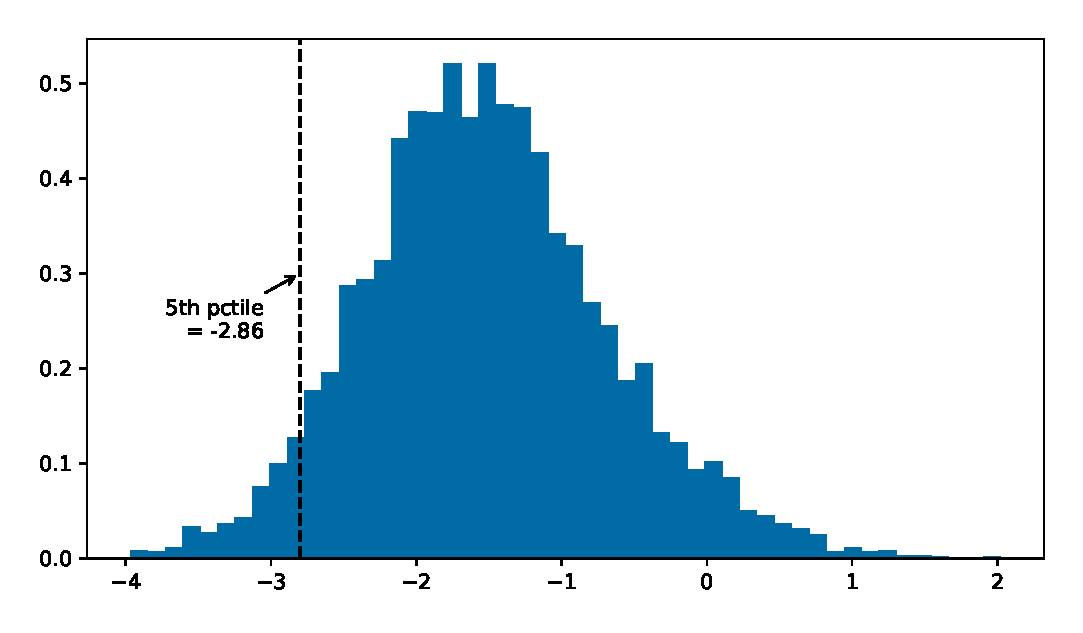
\includegraphics[width=\linewidth]{fig/dickey_fuller.eps} \\
\vspace{-\baselineskip}
\[y_t = y_{t-1} + u_t,\quad u_t \overset{iid}{\sim} N(0,1),\quad T=1000,\quad 5000 \text{ simulations}\]
\end{figure}
}

\frame{
\frametitle{Unit root test: AR($p$)}
\begin{itemize}
\item Consider testing for a unit root in a more general AR($p$) model
\[y_t = c + a_1 y_{t-1} + \dots + a_p y_{t-p} + u_t.\]
\item \alert{Exercise:} show that we can rewrite this model as
\[y_t = c + \rho y_{t-1} + \gamma_1 \Delta y_{t-1} + \dots + \gamma_{p-1} \Delta y_{t-p+1} + u_t,\]
where $\rho \equiv \sum_{\ell=1}^p a_\ell$ and $\gamma_\ell \equiv -\sum_{j=\ell+1}^p a_j$.
\item We've seen that we have a unit root if and only if $\rho\equiv \sum_{\ell=1}^p a_\ell=1$.
\end{itemize}
}

\frame{
\frametitle{Unit root test: AR($p$) (cont.)}
\begin{itemize}
\item \textbf{Augmented Dickey-Fuller} (ADF) t-test:
\begin{enumerate}
\item Select lag length $p$ (e.g., AIC).
\item OLS regression:
\[y_t = \hat{c} + \hat{\rho} y_{t-1} + \hat{\gamma}_1 \Delta y_{t-1} + \dots + \hat{\gamma}_{p-1} \Delta y_{t-p+1} + \hat{u}_t.\]
\item Compute t-statistic with homoskedastic OLS SE:
\[\hat{t} \equiv \frac{\hat{\rho}-1}{\mathit{SE}(\hat{\rho})}.\]
\item Reject null hypothesis of unit root (without drift) if $\hat{t} < \mathit{cv}_\alpha$.
\end{enumerate}
\item It turns out that $\hat{t}$ has the same null distribution as in the AR(1) case earlier. So the 5\% critical value $\mathit{cv}_{0.05}$ remains $-2.86$.
\begin{itemize}
\item See Stock \& Watson, chapter 15.7, for 1\% and 10\% crit.\ values.
\end{itemize}
\end{itemize}
}

\frame{
\frametitle{Unit root test: AR($p$) (cont.)}
\begin{itemize}
\item Some papers/software use an alternative but equivalent formulation of the ADF t-test.
\item Suppose we run an ADF regression, but with the dependent variable in first differences rather than levels:
\[\alert{\Delta y_t} = \hat{c} + \hat{\delta} y_{t-1} + \hat{\gamma}_1 \Delta y_{t-1} + \dots + \hat{\gamma}_{p-1} \Delta y_{t-p+1} + \hat{u}_t.\]
\item By the linearity of OLS, $\hat{\delta} = \hat{\rho}-1$ (exactly).
\item So with this regression specification, the ADF test statistic should be for the hypothesis $\alert{\delta=0}$ (not 1).
\item Critical value unchanged, of course.
\end{itemize}
}

\begin{frame}[fragile]
\footnotesize
\begin{verbatim}
# Manual ADF test
p = 4
dy = np.diff(y) # GDP growth

X_adf = pd.DataFrame(
    np.column_stack([y[p-1:-1], lagmat(dy, p-1, trim='both')]),
    columns=['y_lag1'] + [f'Dy_lag{k}' for k in range(1, p)],
)
X_adf = sm.add_constant(X_adf)
res_adf = sm.OLS(pd.Series(dy[p-1:], name='dy'), X_adf).fit()
print(res_adf.summary())
\end{verbatim}
\end{frame}

\begin{frame}[fragile]
\scriptsize
\begin{verbatim}
                            OLS Regression Results                            
==============================================================================
Dep. Variable:                     dy   R-squared:                       0.043
Model:                            OLS   Adj. R-squared:                  0.031
Method:                 Least Squares   F-statistic:                     3.490
Date:                Fri, 15 May 2026   Prob (F-statistic):            0.00833
Time:                        15:39:35   Log-Likelihood:                 969.17
No. Observations:                 312   AIC:                            -1928.
Df Residuals:                     307   BIC:                            -1910.
Df Model:                           4                                         
Covariance Type:            nonrobust                                         
==============================================================================
                 coef    std err          t      P>|t|      [0.025      0.975]
------------------------------------------------------------------------------
const          0.0248      0.008      2.949      0.003       0.008       0.041
y_lag1        -0.0020      0.001     -2.230      0.026      -0.004      -0.000
Dy_lag1        0.1092      0.057      1.919      0.056      -0.003       0.221
Dy_lag2        0.0886      0.057      1.556      0.121      -0.023       0.201
Dy_lag3       -0.0418      0.057     -0.738      0.461      -0.153       0.070
==============================================================================
\end{verbatim}
\uncover<2>{%
\begin{tikzpicture}[overlay, remember picture]
  \circleoverlay[cx=0.15cm, cy=-1.25cm, r=0.6cm,
                 tx=-1.2cm, ty=0.9cm, text anchor=south]{$\hat{t}>-2.86$, so can't \\ reject unit root}
\end{tikzpicture}
}
\uncover<3>{%
\begin{tikzpicture}[overlay, remember picture]
  \circleoverlay[cx=1.85cm, cy=-1.25cm, r=0.5cm,
                 tx=-1.1cm, ty=-0.8cm, text anchor=north]{Ignore this! \\ (assumes normality)}
\end{tikzpicture}
}
\end{frame}

\begin{frame}[fragile]
\scriptsize
\begin{verbatim}
from statsmodels.tsa.stattools import adfuller

print('Null: RW no drift, alternative: stationary')
adf_stat, p_val, *_ = adfuller(y, maxlag=p-1, regression='c', autolag=None)
print(f't-stat: {adf_stat:.4f}, p-value: {p_val:.4f}')
\end{verbatim}
\bigskip
\normalsize
\textbf{Results:}
\smallskip
\scriptsize
\begin{verbatim}
Null: RW no drift, alternative: stationary
t-stat: -2.2305, p-value: 0.1954
\end{verbatim}
\uncover<2>{%
\bigskip
\normalsize
Note: \texttt{maxlag} = number of lagged first differences $\Delta y_{t-\ell}$ in the regression
\begin{tikzpicture}[overlay, remember picture]
  \circleoverlay[cx=-4.1cm, cy=-0.5cm, r=0.6cm,
                 tx=0.8cm, ty=0.8cm, text anchor=west]{Same as previous slide}
\end{tikzpicture}
}
\end{frame}

\frame{
\frametitle{ADF test with clearly trending data}
\begin{itemize}
\item The ADF test on the preceding slides tests the null hypothesis of a random walk \emph{without} drift against the alternative of \emph{stationarity}.
\item This test does not make much sense if the data has a very clear positive or negative time trend.
\item Instead, consider testing the null hypothesis of a random walk \emph{with} drift against the alternative of \emph{trend} stationarity. Then we need to add a time trend to the ADF regression:
\[\Delta y_t = \hat{c} + \alert{\hat{\zeta}t} + \hat{\delta} y_{t-1} + \hat{\gamma}_1 \Delta y_{t-1} + \dots + \hat{\gamma}_{p-1} \Delta y_{t-p+1} + \hat{u}_t.\]
\item Compute the t-statistic for $\delta=0$. Limiting distribution under the null differs from before. Critical values: Stock \& Watson, chapter 15.7.
\end{itemize}
}

\begin{frame}[fragile]
\scriptsize
\begin{verbatim}
print('Null: RW w/drift, alternative: trend stationary')
adf_stat2, p_val2, *_ = adfuller(y, maxlag=p-1, regression='ct', autolag=None)
print(f't-stat: {adf_stat2:.4f}, p-value: {p_val2:.4f}')
\end{verbatim}
\bigskip
\normalsize
\textbf{Results:}
\smallskip
\scriptsize
\begin{verbatim}
Null: RW w/drift, alternative: trend stationary
t-stat: -1.6259, p-value: 0.7821
\end{verbatim}
\bigskip
\normalsize
{\tt regression='c'}: no time trend, just intercept \\
{\tt regression='ct'}: include time trend
\end{frame}


\frame{
\frametitle{Near-unit roots}
\begin{itemize}
\item In data of a given sample size $T$, there is little difference between an AR($p$) process with $\rho = 1$ and one with $\rho=0.999$, say.
\begin{itemize}
\item Recall $\rho \equiv \sum_{\ell=1}^p a_\ell$.
\end{itemize}
\item So if we have a root very \emph{close} to 1, normality-based statistical procedures could behave poorly (unless $T$ is astronomically large).
\item The case $\rho \approx 1$ requires as much attention as $\rho=1$.
\item You might hope that the bootstrap could help us adapt to the magnitude of $\rho$, but unfortunately not when $\rho \approx 1$.
\begin{itemize}
\item Intuition: the bootstrap generates fake data based on the severely downward-biased OLS estimate $\hat{\rho}$ of $\rho$. So the bootstrap is ``too optimistic'' about how normally distributed $\hat{\rho}$ is.
\end{itemize}
\end{itemize}
}

\frame{
\frametitle{Dealing with unit roots in practice}
\begin{itemize}
\item When researchers are unsure about how to model a potentially trending series $\lbrace y_t \rbrace$, it's common to proceed in steps:
\begin{itemize}
\item Run ADF test.
\item Reject unit root $\Rightarrow$ estimate stationary model for $\lbrace y_t \rbrace$.
\item Fail to reject unit root $\Rightarrow$ estimate stationary model for $\lbrace \Delta y_t \rbrace$.
\end{itemize}
\item But the first-step \textbf{pre-test} will sometimes commit a type-I or type-II error, which can mess up later inference.
\end{itemize}
}

\frame{
\frametitle{Dealing with unit roots in practice (cont.)}
\begin{itemize}
\item If we don't care about the presence of a unit root \emph{per se}, it's often better to skip the pre-test and just estimate the AR model in \emph{levels} (or log levels):
\[y_t = \hat{c} + \hat{a}_1 y_{t-1} + \dots + \hat{a}_p y_{t-p} + \hat{u}_t.\]
\item If the true process has a unit root, then $\hat{\rho} \equiv \hat{a}_1 + \dots + \hat{a}_p$ has a non-normal distribution, as we've seen.
\item But if the lag order $p>1$, the individual coefficients $\hat{a}_\ell$ typically have (asymptotic) normal distributions, so we can use conventional normality-based tests and confidence intervals for these.
\item Moreover, impulse responses -- which are functions of the coefficients -- are also usually normally distributed.
\item These conclusions extend to VARs: just use variables in (log) levels.
\end{itemize}
}

\frame{
\frametitle{Dealing with unit roots in practice (cont.)}
\begin{itemize}
\item A Bayesian who is confident in her prior need not be concerned about unit roots.
\item There is nothing in our likelihood calculation that depends on stationarity. So posterior inference can proceed as usual.
\item But results could be quite sensitive to the choice of prior if some roots are close to 1.
\end{itemize}
}

\frame{
\frametitle{What did we learn?}
\begin{itemize}
\item Trend stationarity
\item Stochastic trend, random walk
\item AR model with unit root
\begin{itemize}
\item Super-consistent OLS estimator
\item Non-normal estimator and t-statistic
\end{itemize}
\item ADF test for unit root
\item Often best to avoid pre-tests and just estimate the AR/VAR in (log) levels
\end{itemize}
}

\frame{
\frametitle{Looking ahead}
\begin{itemize}
\item Modeling multiple time series with common trends
\item Testing for structural breaks
\item Removing trends and seasonality from data
\end{itemize}
}

\end{document}